\setchapterpreamble[u]{\margintoc}
\chapter{Answers}
\labch{ch-answers}


Tasks and questions are scattered throughout the book, 
and the answers are collected in this chapter.


\section{Introduction}
\labsec{answer-intro}


\begin{exercise}%
    \label{answer:short-link-to-SPARQL}
How to create a short link to a SPARQL script?
\end{exercise}

\begin{marginfigure}[0cm]
    {%
        \setlength{\fboxsep}{0pt}
        \setlength{\fboxrule}{1pt}
        \fcolorbox{gray}{gray}{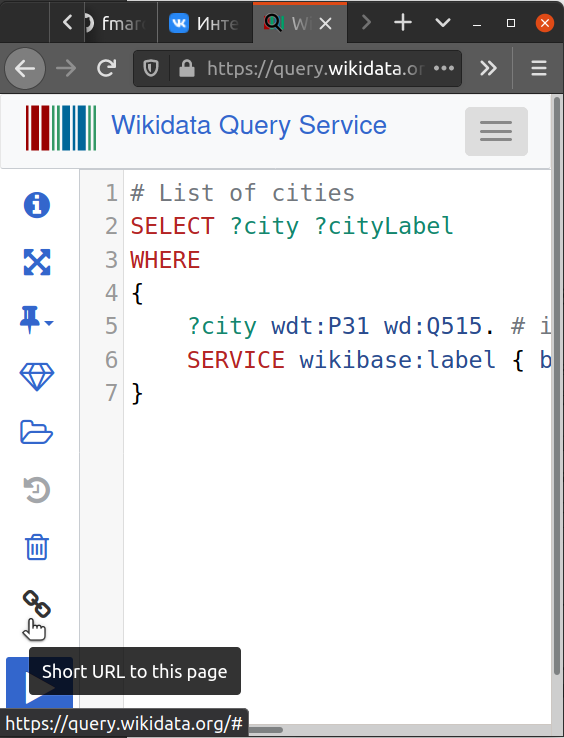
\includegraphics[width=\linewidth]{chapter/intro/WD_Query_Service_Short_URL_2020.png}}
    }
	\caption{The chain symbol button creates a short link to the SPARQL script, Wikidata Query Service, 2020.}
	\labfig{fig:WDQS-Short-URL-creation}
\end{marginfigure}

The Wikidata Query Service is shown in~\reffig{fig:WDQS-Short-URL-creation}. 
The bottom button with a chain symbol allows you to create a short link to the SPARQL script. 

See question on page~\pageref{question:short-link-to-SPARQL}.



\section{Aircraft from small to large}
\labsec{answer-aircraft}

\begin{exercise}%
    \label{answer:formulate-your-short-label-for-question-here-please}
Question one?
\end{exercise}

Answer text.



\section{From towns to cities with millions of inhabitants}
\labsec{answer-towns}

\begin{exercise}%
    \label{answer:formulate-your-short-label-for-question-here-please2}
Question two?
\end{exercise}

Answer text.


